\documentclass[10pt,pscyr,nonums]{hedlab}
\usepackage[russian]{babel}
\usepackage{hedmaths}
\usepackage{graphicx}
\graphicspath{{images/}, {plots/}}

\newgeometry{top=1.5cm, bottom=1.5cm, left=1cm, right=1cm}

\student{Слоква В. И., Ф-469}
\date{16.10.2013}
\labnum{502}
\labname{Изучение законов внешнего фотоэффекта}

\begin{document}
  \makeheader

  \emph{Цель работы:} практическое ознакомление с закономерностями внешнего
  фотоэффекта; экспериментальное определение работы выхода электрона из
  сурьмяно-цезиевого фотокатода, красной границы фотоэффекта, а также
  постоянной Планка.
  
  \emph{Используемые при расчетах формулы:}
  \( \omega = 2\pi c/\lambda; \ \hbar = eU_*/\omega_0; \ A_0 = \hbar\omega_0 \).

  \begin{figure}[h!]
    \center
    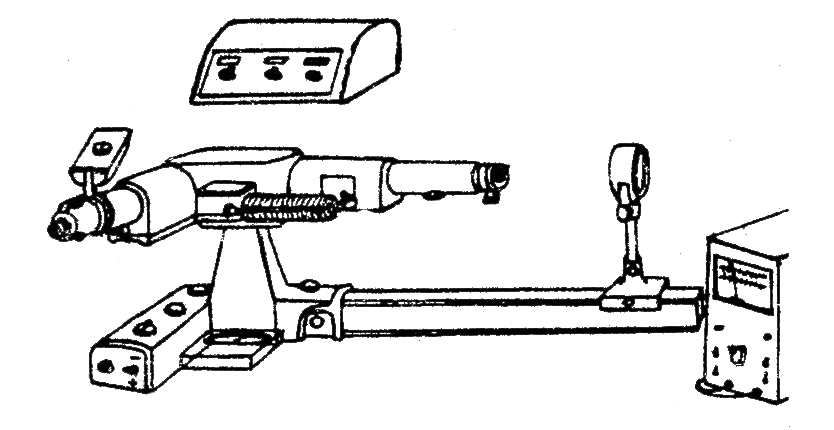
\includegraphics[width=.4\textwidth]{appearance} \hspace*{2em}
    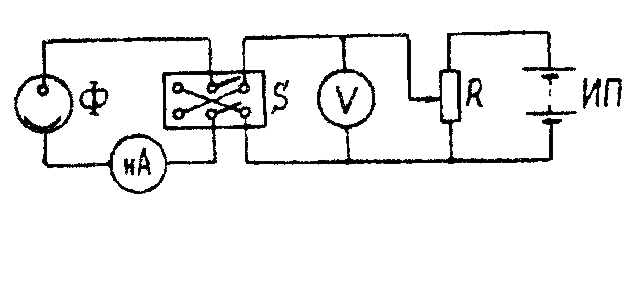
\includegraphics[width=.4\textwidth]{scheme} \\[.5em]
    \parbox{.4\textwidth}{\caption{Внешний вид установки}} \hspace*{2em}
    \parbox{.4\textwidth}{\caption{Схема подключения фотоэлемента}}
  \end{figure}
  \vspace*{-2em}
  
  \begin{table}[h!]
    \center \caption{Измерение запирающего напряжения}
    \begin{tabular}{|*{2}{C{.12}|}*{4}{C{.07}|}} \hline
      \multirow{2}{*}{Длина волны} &
        \multirow{2}{*}{Частота} &
        \multicolumn{4}{c|}{Задерживающее напряжение} \\ \cline{3-6}
      && \multicolumn{3}{c|}{\( U_\text{з} \)} &
        \( \midnum{U_\text{з}} \) \\ \hline
      Нм & \( 10^{15}~\text{с}^{-1} \) &
        В & В & В & В \\ \hline
      404,7 & 4,66 & 0,76 & 0,76 & 0,80 & 0,77 \\ \hline
      435,6 & 4,33 & 0,72 & 0,72 & 0,68 & 0,71 \\ \hline
      546,6 & 3,45 & 0,48 & 0,48 & 0,48 & 0,48 \\ \hline
    \end{tabular}
  \end{table}
  
  \begin{table}[h!]
    \center \caption{Вольт-амперные характеристики фотокатода}
    \begin{tabular}{|C{.12}|*{7}{C{.05}|}} \hline
      Длина волны \( \lambda \),~нм &
        \( U \),~В & 0 & 0,6 & 1,2 & 1,8 & 2,4 & 3,0 \\ \hline
      404,7 & \( I \),~нА &  7,2 &  8,6 &  9,6 & 21,0 & 22,2 & 22,8 \\ \hline
      435,6 & \( I \),~нА & 19,2 & 24,6 & 30,0 & 70,0 & 74,0 & 76,0 \\ \hline
      546,6 & \( I \),~нА & 58,0 & 66,0 & 72,0 & 74,0 & 78,0 & 80,0 \\ \hline
    \end{tabular}
  \end{table}
  
  \begin{table}[h!]
    \center \caption{Однократные измерения}
    \begin{tabular}{|*{6}{C{.12}|}} \hline
      \multirow{3}{*}{\( \omega_0 \), \( 10^{15}~\text{с}^{-1} \)} &
        \multirow{3}{*}{\( U_* \),~В} &
        \multicolumn{2}{c|}{\multirow{2}{*}{Работа выхода \( A_0 \)}} &
        Красная & Постоянная \\
      && \multicolumn{2}{c|}{} &
        граница & Планка \\ \cline{3-4}
      && \( 10^{-19} \)~Дж & эВ &
        \( \lambda_0 \),~нм &
        \( \hbar \),~Дж\(\cdot\)с \\ \hline
      1,1 & -0,34 & 0,544 & 0,34 & 1712,41 &
        \( 4,\!945 \cdot 10^{-35} \) \\ \hline
    \end{tabular}
  \end{table}
\end{document}
